\section{Motivation}

\yueqiang{Key Observation 1: Page type updates have impacts on the IOTLB miss, and thereby affect I/O performance}
\yueqiang{To serve the first observation, we need 7 page types and their update graph. Any update needs a corresponding validation $->$ IOTLB flush.}

\yueqiang{Key Observation 2: The main source of the page type update is from writable-to-pagetable page update.}
\yueqiang{To serve the second observation, we need 7 page types and their update graph. All other updates are only once in the whole life cycle, while the writable-pagetable page updates are frequent.}

By analysing how Xen validates the update of page type, we have uncovered the relationship between page type update and I/O TLB flush . Here We use a specific update from writable to page-table to illustrate the relationship in detail.

Every time a guest OS launches a new process, it creates a new multi-level page table, multiple pages of which are allocated from the buddy system and initialized by OS. At the time, OS fills up the pages of writable-type with entries mapping virtual addresses to the machines addresses and submits update requests to Xen.

Since the pages are writable and their type reference counts are not zero at the moment, Xen firstly reduces the count to zero and then vets every entry in every level of page tables through a page table walk. If there exists an entry pointing to a machine page beyond the OS, then the update fails. If not, Xen will set and pin every page to its corresponding page-table type. The pinning mechanism is used to avoid performance cost. Specifically, each time Xen installs a new page table base pointer to the control register CR3 (i.e., context switch), it does not have to validate the page tables if they are pinned.

In the meantime, Xen must clear \emph{read} and \emph{write} permission fields in the I/O page tables corresponding to the machine frames of guest page tables and flush specified IOTLB entries. To achieve high performance while ensure safety, Xen requires multiple page-selective invalidations utilizing queued invalidation interface. Figure \ref{fig:wr2pt} describes the page type updates of machine pages between these two page types.

\begin{figure}[ht]
\centering
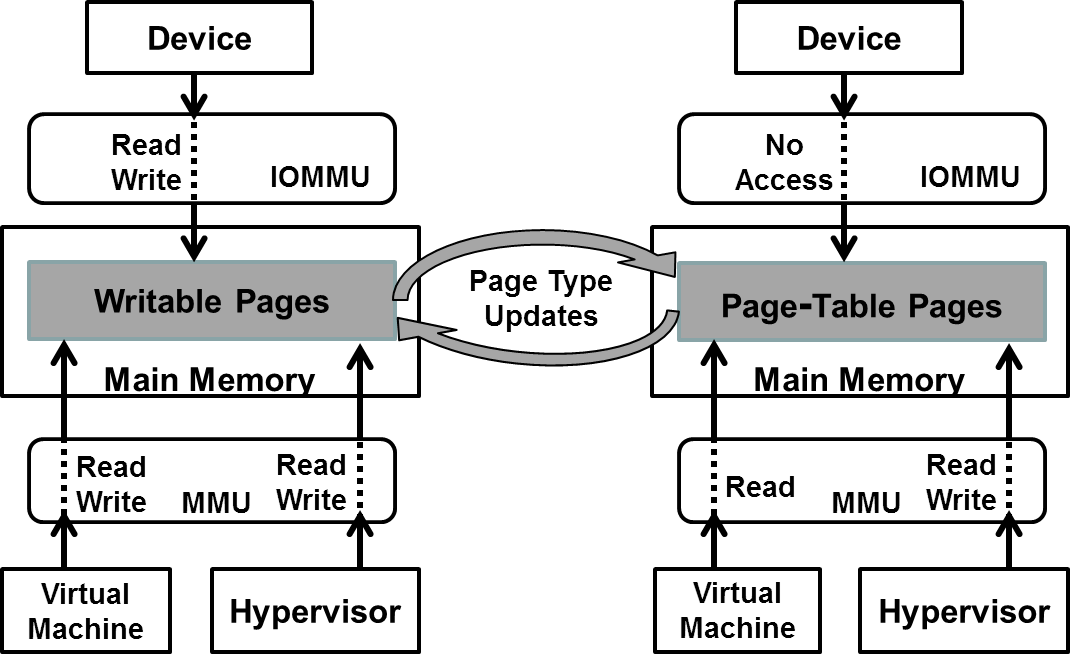
\includegraphics[width=0.5\textwidth]{image/background/wr2pt.png} \\
\caption{Page Type Updates Between Writable and Page-Table}
\label{fig:wr2pt}
\end{figure}

From the description above, we have two key observations as follows:

1. Every page type update in figure \ref{fig:page-type-update} will force Xen to map or unmap a specific page from I/O page table and thus flush a corresponding IOTLB entry, which may have a bad impact on I/O performance.

2. Among all the page type updates, the update between writable and page-table is the main source of causing IOTLB-flush, since page table creation/destruction is very common during runtime while GDT/LDT creation/destruction is rare.

Based on the observations, we are motivated to propose a novel algorithm for guest OS to manage page tables in order to reduce as many IOTLB flushes as possible for a maximum possible use of the IOTLB-path while retain the safety.
